\chapter{Ebner Data} \label{cha:real-world-application}

We will now apply the concept of shape-constraint P-splines onto real-life data to incorporated a priori domain knowledge into the fitting process. The data is generated from a heat treatment process of aluminum. The aluminum is heated up to a specific temperature, hold at this temperature for some predefined time and then cooled using water jets. This controlled heating and cooling enhances structural properties of the aluminum. Our interest lies on the cooling phase, since it is a highly non-linear process due to phase changes of the cooling medium and therefore difficult to model using first-principle methods. Nevertheless, we can use these in the form of a priori domain knowledge. To model the cooling phase, we try to estimate the heat transfer coefficient, i.e.

\begin{align}
	\alpha := \alpha(T, \dot m),
\end{align}
%
as a function of the temperature $T$ of the aluminum and the mass flow $\dot m$ of the cooling medium. We know beforehand, that the heat transfer coefficient $\alpha$ may only increase when increasing the mass flow $\dot m$ and that it shows unimodal peak behavior for increasing temperature $T$, motivated by the so-called Leidenfrost effect. 

The data situation is visualized in Figure \ref{fig:ebner_data_situation}. Here we show how many data points are given in a area of approximately $50 K$ and $0.9 [kg/s]$. We have some regions, where no data is available, while the majority of data points is located in small areas. This is a problem, which is often encountered in real-world situations. 

\begin{figure}[H]
	\centering
	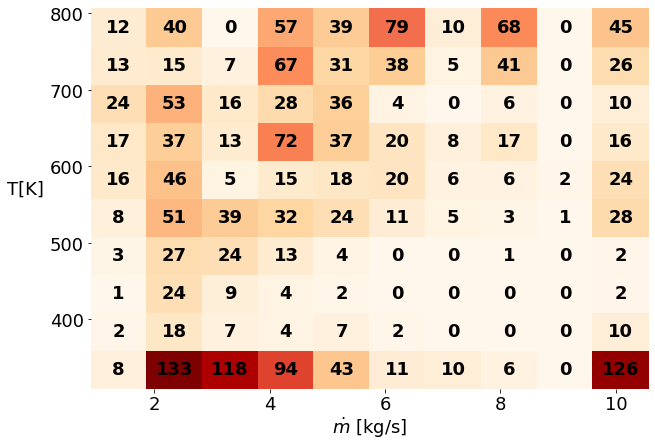
\includegraphics[width=\columnwidth]{graphics/pgfplots/cha5/data_distribution.png}
	\caption{Data Situation}
	\label{fig:ebner_data_situation}
\end{figure}

This may lead to some difficulties when using B-splines and tensor-product B-splines, as they do not handle sparse data situations well, cf.~\pref{cha:practical-considerations}. Nevertheless, using regularization should help to cope the data situation. 

We will now use various models using B-splines, tensor-product B-splines and their shape-constraint alternatives to recover a model for the heat transfer coefficient given the data. The following list describes the models.

\begin{enumerate}[(i)] \label{Model-List}
	\item M1 $= s(1) + s(2)$
	\item M2 $= s(1) + s(2)$, using monotonicity for $s(1)$ and unimodal peak behavior for $s(2)$
	\item M3 $= t(1,2)$
	\item M4 $= t(1,2)$, using monotonicity for dimension $1$
	\item M5 $= s(1) + s(2) + t(1,2)$, as additive model using $(\text{i})$ and $(\text{iii)}$
	\item M6 $= s(1) +s(2) + t(1,2)$, as additive model using $(\text{ii})$ and $(\text{iv})$
\end{enumerate}

To fit the models listed in \ref{Model-List}, we perform a randomized train-validation split on the data, i.e. we split the data into a training set $\mathcal{D}_{\text{train}}$ and a validation set $\mathcal{D}_{\text{val}}$, fit the models to the resulting training set and evaluate its performance by calculating the mean squared error on the validation set as well as by visual inspection. We choose to split the data into sets of the same size since it is quite noise and we therefore hope to generate a more stable estimation of the prediction error for previously unseen data. A visual inspection of the of the data distribution given by the train-validation split is given in~\pref{fig:ebner-train-val-split}.

\begin{figure}[H]
	\centering
	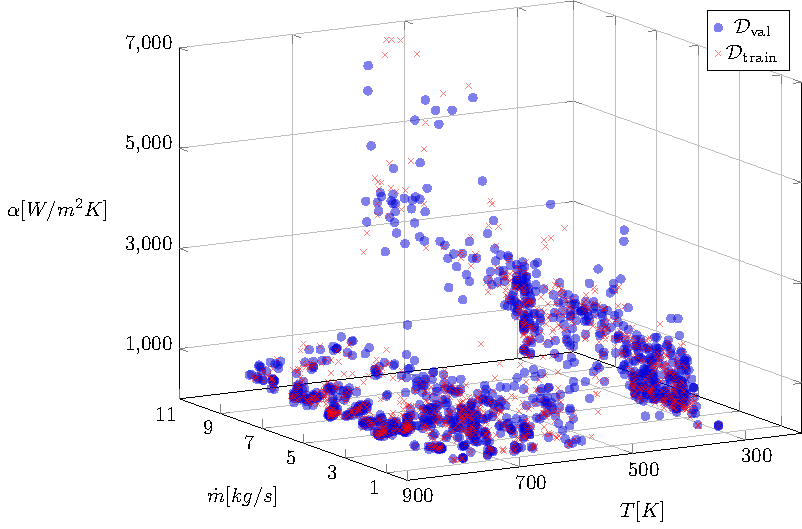
\includegraphics[width=\columnwidth]{graphics/pgfplots/cha5/train-val-split.pdf}
	\caption{Training set $\mathcal{D}_{\text{train}}$ and validation set $\mathcal{D}_{\text{val}}$.}
	\label{fig:ebner-train-val-split}
\end{figure}
%
The mean squared errors evaluated on the validations set is given in~\pref{tab:ebner-mse-val}. According to these, the best model is M4, i.e. the shape-constraint tensor-product B-spline with a monotonicity constraint in the mass flow dimension. The models M3, i.e. the tensor-product B-spline, and M6, i.e. the additive model using shape constraints, perform nearly as well as M4 according to the mean squared error on the validation set. 

\begin{table}[H]
	\begin{center}
		\pgfplotstabletypeset[
		col sep=comma,
		columns/Model/.style={string type},
		columns/MSE_val/.style={column name={$\text{MSE}_{\text{val}}$}},
		every head row/.style={before row=\toprule[1pt] \toprule,after row=\midrule[2pt]},
		every last row/.style={after row=\bottomrule \bottomrule},
		every nth row={1}{before row=\midrule},
		]{graphics/data/cha5/mses.csv}
	\end{center}
	\caption{Mean squared errors on the validation set $\mathcal{D}_{\text{val}}$.}
	\label{tab:ebner-mse-val}
\end{table}

The predictions for model M4 are shown in~\pref{fig:ebner-M4}. The peak behavior in the temperature dimension is clearly visible, as well as an increasing trend within the massflow dimension. Therefore, we conclude that model M4 is the superior model with regards to the domain knowledge and data fidelity. 

\begin{figure}[H]
	\centering
	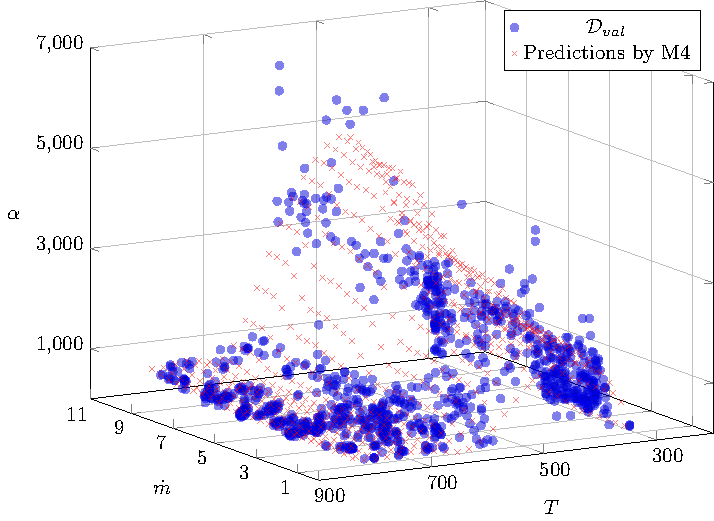
\includegraphics[width=\columnwidth]{graphics/pgfplots/cha5/M4.pdf}
	\caption{Validation set $\mathcal{D}_{\text{val}}$ and predictions by model M4.}
	\label{fig:ebner-M4}
\end{figure}

The predictions for model M6 are shown in~\pref{fig:ebner-M6}. Here, the peak behavior can also be identified, but in a weaker fashion as for model M4 in~\pref{fig:ebner-M4}. We also obtain an increasing trend in the massflow dimension. 

\begin{figure}[H]
	\centering
	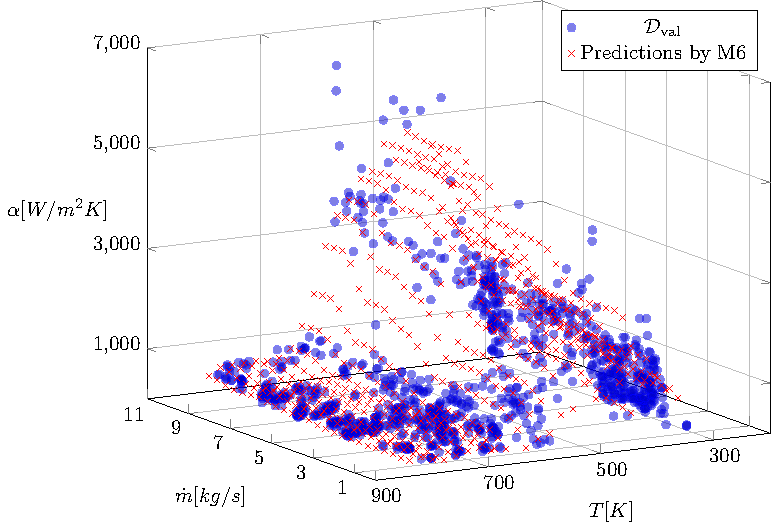
\includegraphics[width=\columnwidth]{graphics/pgfplots/cha5/M6.pdf}
	\caption{Validation set $\mathcal{D}_{\text{val}}$ and predictions by model M6.}
	\label{fig:ebner-M6}
\end{figure}
%
The visual inspection of the predictions of model M3 in~\pref{fig:ebner-M3} indicates that there is massive overfitting present. Neither smooth, nor the a priori known behavior (increasing in the massflow dimension and a peak behavior in the temperature dimension) is identifiable.  

\begin{figure}[H]
	\centering
	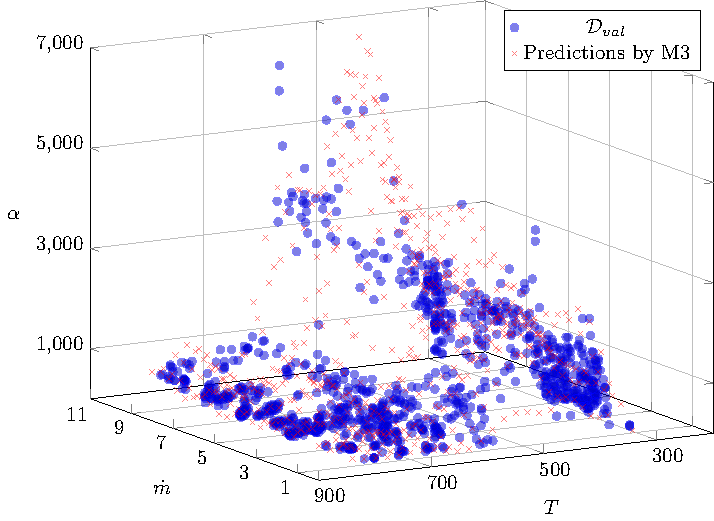
\includegraphics[width=\columnwidth]{graphics/pgfplots/cha5/M3.pdf}
	\caption{Validation set $\mathcal{D}_{\text{val}}$ and predictions by model M3.}
	\label{fig:ebner-M3}
\end{figure}

We omit the visual presentation of the predictions by the models M1, M2 and M5, since for all of these the mean squared errors on the validation set $\mathcal{D}_{\text{val}}$ is at least a magnitude higher, indicating even more severe overfitting. 

To summarized, we see that the incorporation of a priori domain knowledge improves the quality of the fit in all of the above models, e.g. M2 is the better model according to the mean squared error on the validation set $\mathcal{D}_{\text{val}}$ than M1, M4 is better than M3 and M6 is better than M5. Therefore, we conclude that the use of a priori domain knowledge through shape constraints improves the model quality even for real-world data. 
